\documentclass[12pt]{beamer}
\usetheme[navbar=false, bkgimage=false, shadow=true]{Fermi}

\usepackage{graphicx}

\usepackage{amsmath}
\usepackage{xspace}
\usepackage{deluxetable}

\newcommand{\gtlike}{\ensuremath{\mathtt{gtlike}}\xspace}
\newcommand{\pointlike}{\ensuremath{\mathtt{pointlike}}\xspace}
\newcommand{\gtobssim}{\ensuremath{\mathtt{gtobssim}}\xspace}
\newcommand{\fermi}{\textit{Fermi}\xspace}

\title{Search for Spatially Extended \fermi-LAT Sources Using Two Years of Flight
Data}
%\subtitle{\ldots}

\author{Joshua Lande}
\institute{SLAC/Stanford}
\email{joshualande@gmail.com}
\date{August 25, 2011}

\begin{document}

\section{Introduction}

The introduction goes here\ldots


Primary motivations for improved analysis
\begin{itemize}
  \item More data (3 years vs 18 months)
  \item Many new GeV pulsars
  \item Hope to find new PWN in the off-peak emission of \lat-detected \gev Pulsars.
  \item Going to higher energies thanks to improved IRFs.
  \item Better spatial/morphological analysis due to new \pointlike code.
\end{itemize}


\begin{frame}{Fig. 3: Monte Carlo Study of false detection rate}
  \begin{columns}
    \column{.6\textwidth} 
    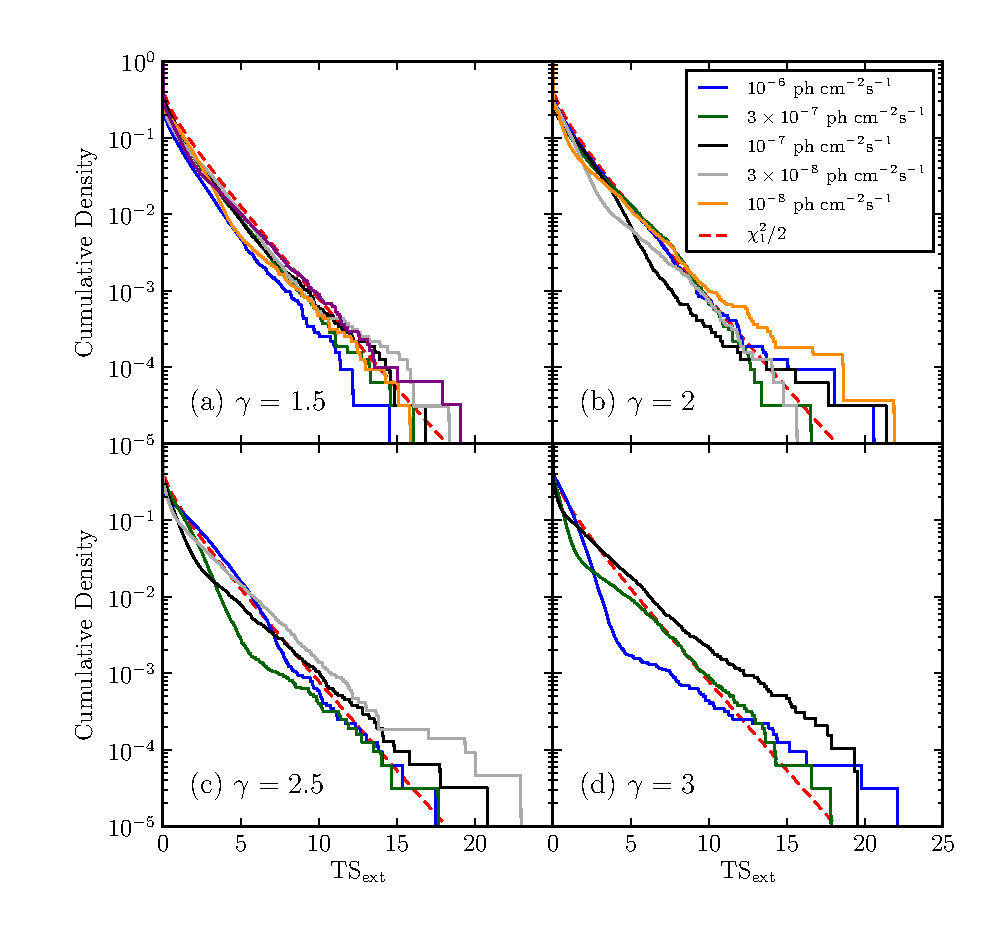
\includegraphics[scale=0.45]{../paper/mc_plots/ts_ext_emin_1000_color.eps}
    \column{.4\textwidth} 
    \begin{itemize}
      \item Test simulated point sources for extension
      \item Lots of spectral parameters
      \item Good agreement with Wilks' Theorem
      \item $\sqrt{\text{TS}_\text{ext}} \rightarrow \# \sigma$
    \end{itemize}
  \end{columns}
\end{frame}



\begin{frame}{Fig. 5: Threshold vs background}
  \begin{columns}
    \column{.6\textwidth} 
    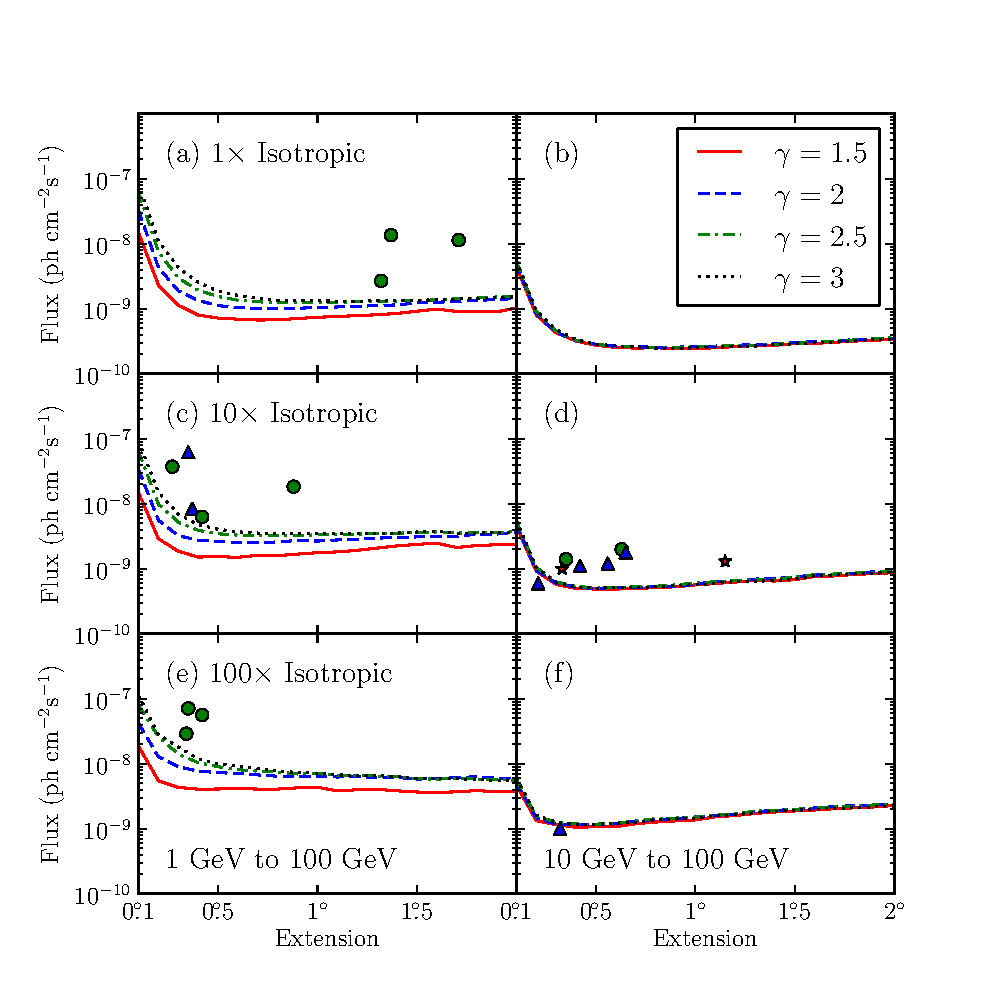
\includegraphics[scale=0.5]{../paper/mc_plots/all_sensitivity_color.eps}
    \column{.4\textwidth} 
    \begin{itemize}
      \item Large Monte Carlo study
      \item Calculate detection threshold
        to spatially extended sources
      \item Overlay LAT extended sources
      \item For future extended sources, can compare to
        threshold
    \end{itemize}
  \end{columns}
\end{frame}

\begin{frame}{Table. 3: Reanalyze 12 sources in 2FGL}
    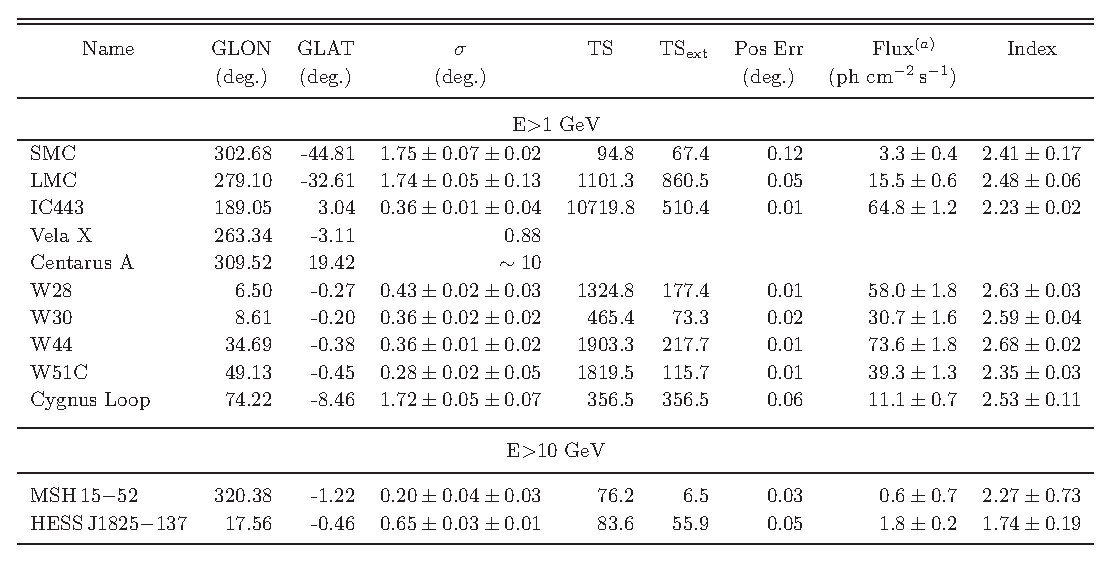
\includegraphics[scale=0.5]{tables/table3.eps}
  \begin{itemize}
    \item Test 12 2FGL sources for extension
    \item But always assume radially symmetric disk spatial model
  \end{itemize}
\end{frame}


\begin{frame}{Table. 4: New Extended Sources}
  \includegraphics[scale=0.45]{tables/table4.eps}
  \begin{itemize}
    \item 9 Extended Sources Not in 2FGL
    \item Skip in this talk
      \begin{itemize}
        \item Vela Jr. - Dedicated Publication
        \item RX\,J1713.7$-$3946 - Dedicated Publication
        \item Ophiuchus - Most likely diffuse emission
      \end{itemize}
  \end{itemize}
\end{frame}

\begin{frame}{Table. 5: Extension Errors}
    \includegraphics[scale=0.5]{tables/table5.eps}
    \begin{itemize}
      \item Two Methods to estimate systematic error on extension
    \begin{itemize}
      \item Alternate diffuse model (add degrees of freedom)
      \item MC representation of the PSF
    \end{itemize}
    \end{itemize}
\end{frame}

\begin{frame}{2FGL\,J0823.0$-$4246 - Puppis A}
  \begin{columns}
    \column{.55\textwidth} 
    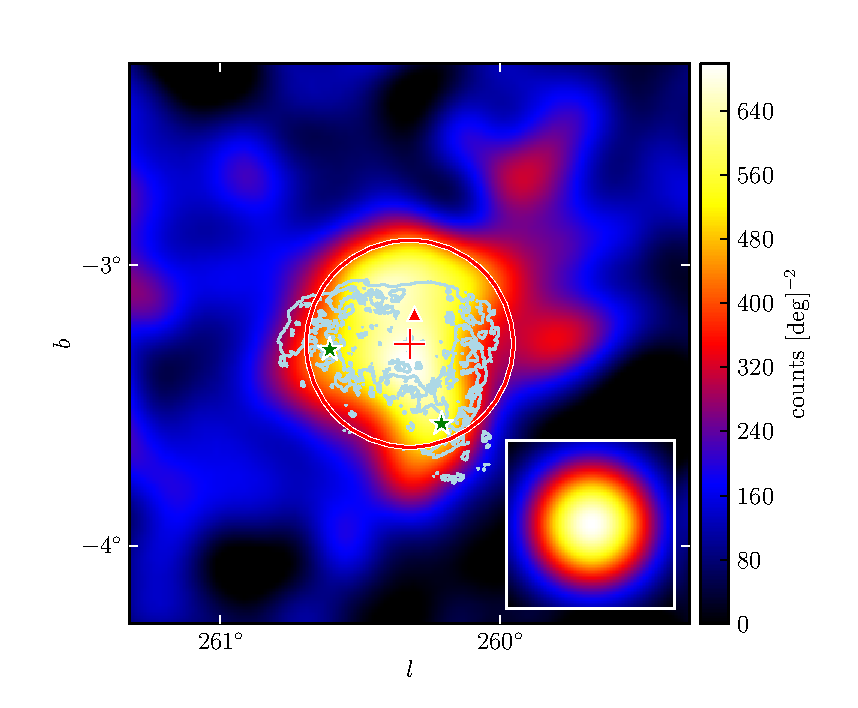
\includegraphics[scale=0.5]{../paper/source_plots/source_Puppis_A_color.eps}
    \column{.45\textwidth} 
    \begin{itemize}
      \item 1 GeV to 100 GeV
      \item Middle-age SNR Puppis A
      \item ROSAT X-ray contours (Petre+1996)
      \item SNR not observed to interact with molecular clouds 
        (Paron+2008)
      \item Similar to Cygnus Loop SNR
    \end{itemize}
  \end{columns}
\end{frame}

\begin{frame}{2FGL\,J2021.5+4026 - $\gamma$-Cygni}
  \begin{columns}
    \column{.55\textwidth} 
    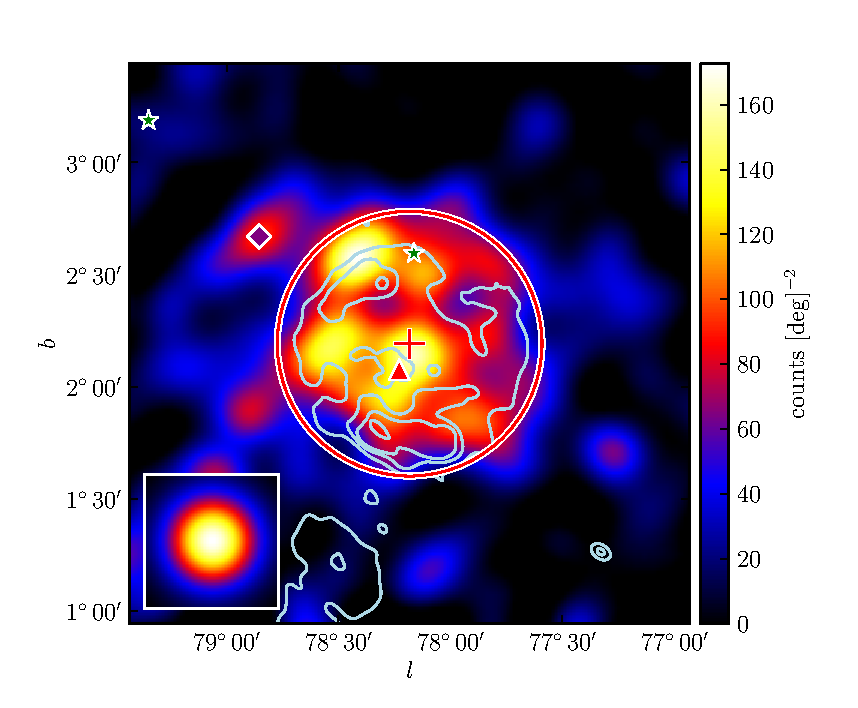
\includegraphics[scale=0.5]{../paper/source_plots/source_Gamma_Cygni_color.eps}
    \column{.45\textwidth} 
    \begin{itemize}
      \item 10 GeV to 100 GeV
      \item PSR\,J2021+4026 at lower energies
      \item Radio contours (Taylor+2003)
      \item SNR interacting with Molecular cloud
      \item Milagro: $4.2\sigma$ excess at $\sim 30$ TeV (Abdo+2009)
      \item 
        VER\,J2019+407 
        detected by Veritas at 200 GeV (Weinstein 2009)
    \end{itemize}
  \end{columns}
\end{frame}


\begin{frame}{Puppis A + $\gamma$-Cygni}
  \begin{center}
    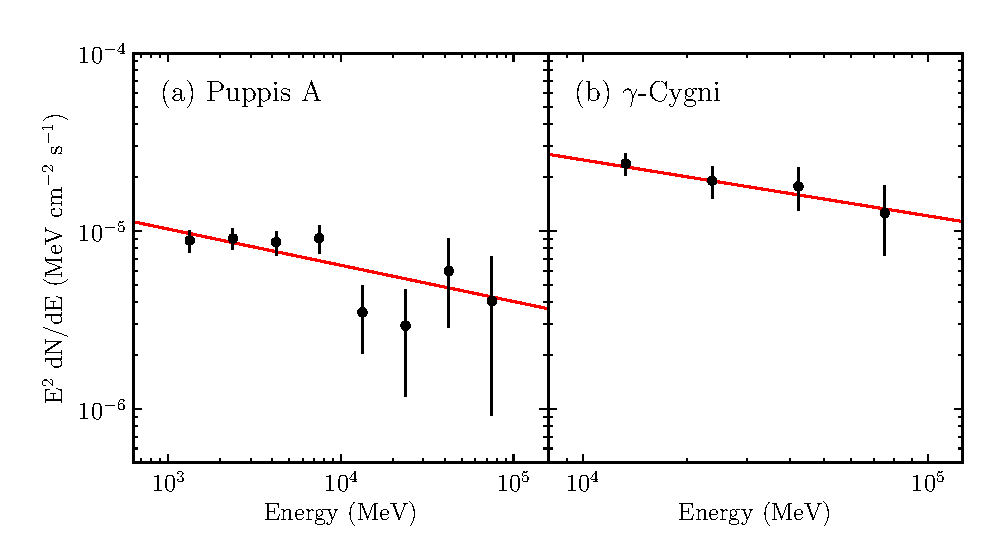
\includegraphics[scale=0.5]{../paper/summary_plots/snr_seds_color.eps}
  \end{center}
\end{frame}

\begin{frame}{HESS\,J1614$-$518 \& HESS\,J1616$-$508}
  \begin{columns}
    \column{.6\textwidth} 
    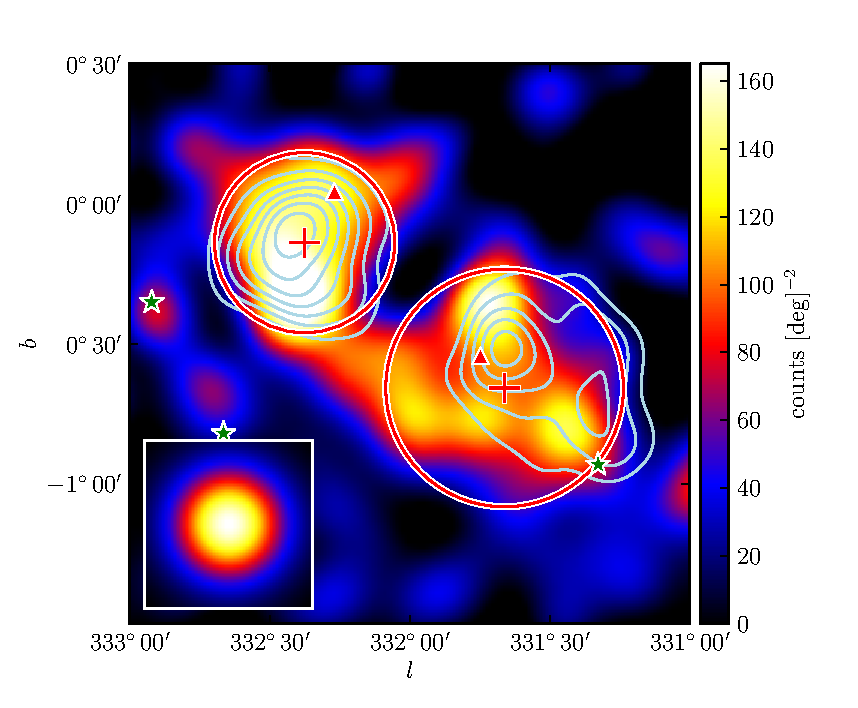
\includegraphics[scale=0.5]{../paper/source_plots/source_HESS_J1614-518_color.eps}
    \column{.4\textwidth} 
    \begin{itemize}
      \item 10 GeV to 100 GeV
      \item Two nearby LAT extended sources 
      \item both
        coincident with extended TeV sources.
    \end{itemize}
  \end{columns}

  \begin{itemize}
    \item (left): 
      2FGL\,J1615.0$-$5051 $\rightarrow$ HESS\,J1616$-$508
    \item (right):
      2FGL\,J1615.2$-$5138 $\rightarrow$ HESS\,J1614$-$518
  \end{itemize}

\end{frame}


\begin{frame}{2FGL\,J1615.0$-$5051 $\rightarrow$ HESS\,J1616$-$508}
  \begin{columns}
    \column{.4\textwidth} 
    % from http://www.mpi-hd.mpg.de/hfm/HESS/pages/home/som/2007/01/
  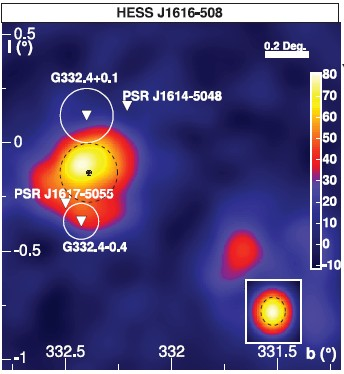
\includegraphics[scale=0.45]{plots/Som_1_07_p1.eps}
    \column{.7\textwidth} 
  \begin{itemize}
    \item 2 nearby SNRs: RCW103 and Kes~32 - not spatially coincident (Aharonian+2006) 
    \item 3 Nearby Pulsars: only 
      PSR\,J1617$-$5055 energetically powerful enough
      \begin{itemize}
        \item 9' away $\rightarrow$ offset PWN?
        \item {\em Chandra} detected $\sim 1'$ PWN 
        \item not oriented towards HESS\,J1616$-$508
        \end{itemize}
      \item Other diffuse emission in region (Kargaltsev+2009)
    \end{itemize}
  \end{columns}
\end{frame}

\begin{frame}{2FGL\,J1615.2$-$5138 $\rightarrow$ HESS\,J1614$-$518}

  \begin{columns}
    \column{.4\textwidth} 
    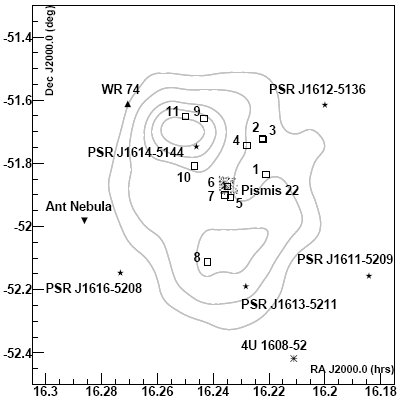
\includegraphics[scale=0.3]{plots/Som_9_08_p1.eps}
    \column{.7\textwidth} 
    \begin{itemize}
      \item 5 nearby pulsars, but none powerful enough (Rowell+2008)
      \item Open cluster Pisim 22 
      \item Suzaku: 2 X-ray sources, one towards peak 
        of HESS\,J1614$-$518 and one coincident with Pisim 22
        (Matsumoto+2008)
      \item SNR? PWN? Acceleration in Stellar Winds of Pisim 22?
    \end{itemize}
  \end{columns}
\end{frame}



\begin{frame}{2FGL\,J1632.4$-$4753c - HESS\,J1632-478}
  \begin{columns}
    \column{.55\textwidth} 
    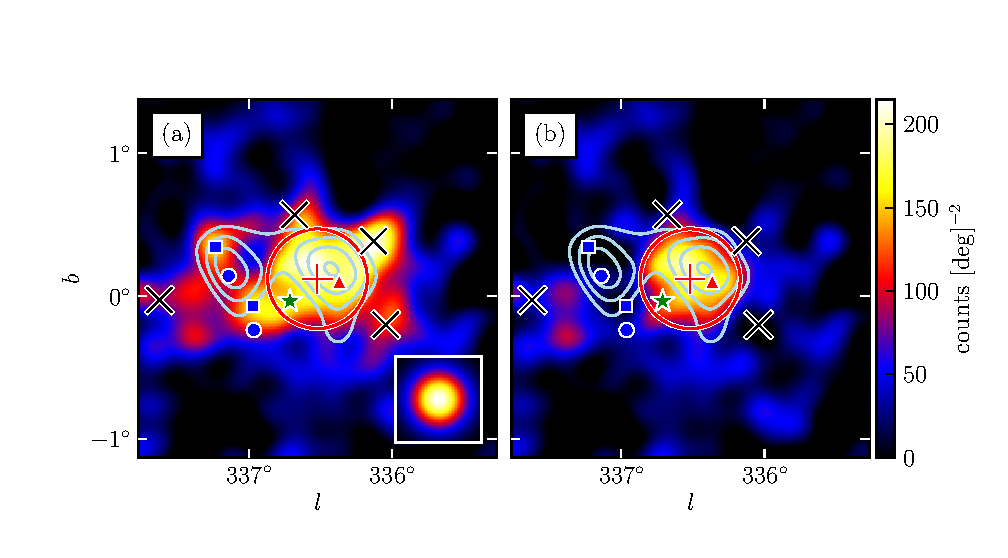
\includegraphics[scale=0.5]{../paper/source_plots/source_HESS_J1632-478_color.eps}
    \column{.45\textwidth} 
    \begin{itemize}
      \item 10 GeV to 100 GeV
      \item  {\em XMM-Newton} point-like + extended emission
        ($32''\times15''$)
        towards center of H.E.S.S source (Balbo+2010)
      \item Extended radio source in archival MGPS-2 data
      \item PWN? No pulsations (yet) in point-like X-ray source
    \end{itemize}
  \end{columns}
\end{frame}

\begin{frame}{2FGL\,J1837.3$-$0700c - HESS\,J1837-069}
  \begin{columns}
    \column{.55\textwidth} 
    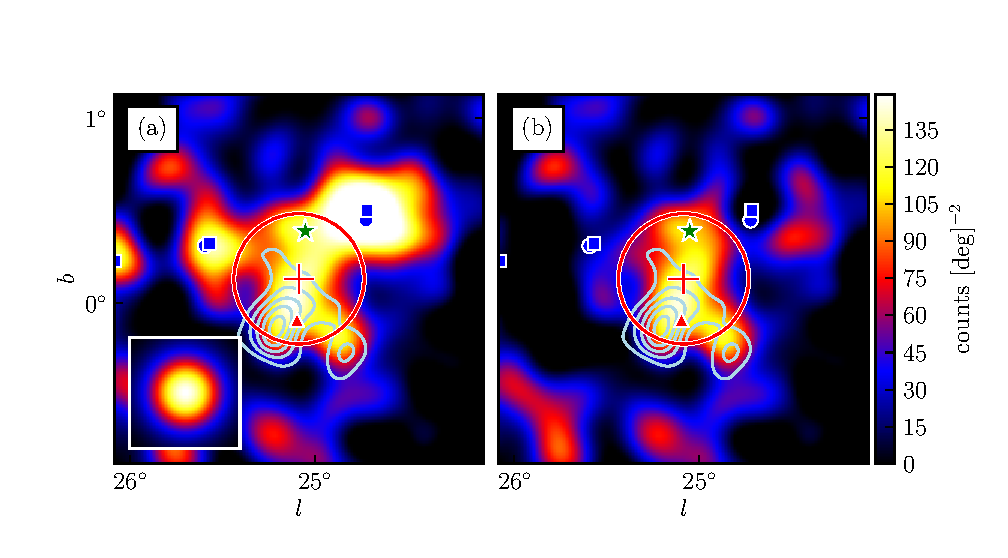
\includegraphics[scale=0.45]{../paper/source_plots/source_HESS_J1837-069_color.eps}
    \column{.45\textwidth} 
    \begin{itemize}
      \item 10 GeV to 100 GeV
      \item Coincident with X-ray source
        AX\,J1838$-$0655 (Hertz \& Grindlay 1988)
      \item X-ray Pulsations: PSR\,J1838$-$0655 
    \end{itemize}
  \end{columns}
    \begin{itemize}
      \item also: X-ray PWN $\sim 2'$ 
        (Gotthelf \& Halpern 2008)
      \item $\gamma$-rays from PWN?
      \item Second X-ray source
        AX\,J1837.3$-$0652 resolved into
        point + extended component (no pulsations yet)
      \item $\gamma$-rays from multiple PWN
    \end{itemize}
\end{frame}

\begin{frame}{LAT + H.E.S.S. SEDs}
  \begin{columns}
    \column{.65\textwidth} 
    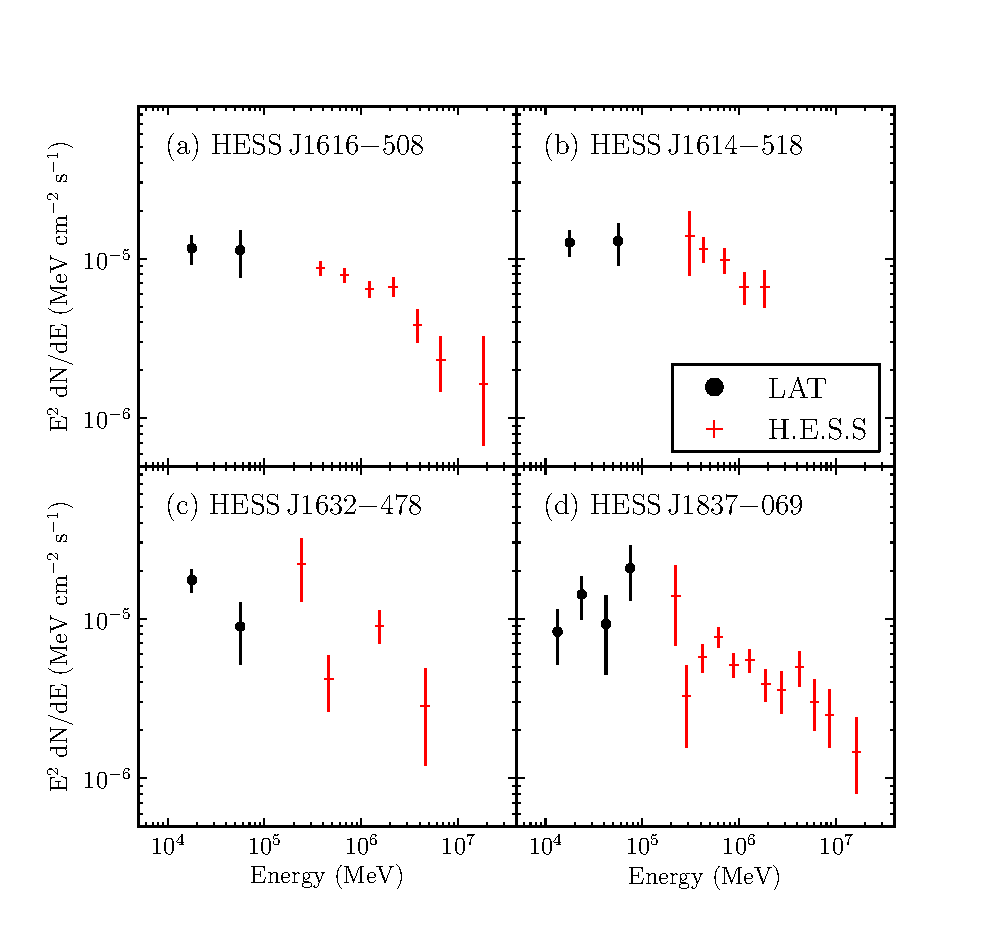
\includegraphics[scale=0.5]{../paper/summary_plots/hess_seds_color.eps}
    \column{.35\textwidth} 
\begin{itemize}
    \item GeV + TeV spectrum connect for
    these souces
  \item (Statistical Errors Only)
  \item
 Future work: take SEDs to lower
    energies
\end{itemize}

  \end{columns}
\end{frame}


\begin{frame}{LAT Detected Extended Sources}
  \begin{center}
    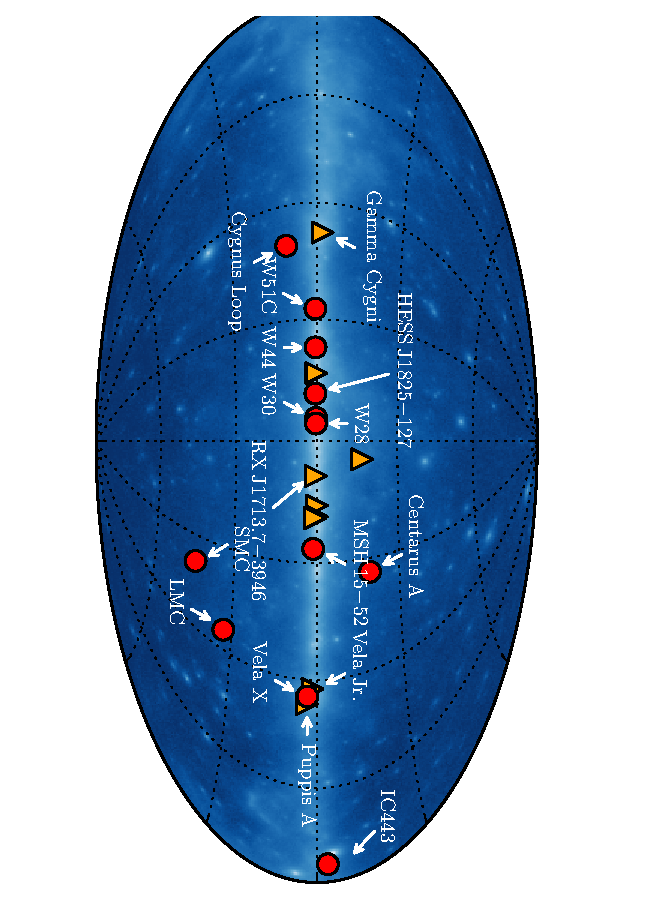
\includegraphics[scale=0.65]{../paper/summary_plots/allsky_extended_sources_color.eps}
  \end{center}
\end{frame}

\begin{frame}{Spectral Index of extended sources}
  \begin{columns}
    \column{.6\textwidth} 
    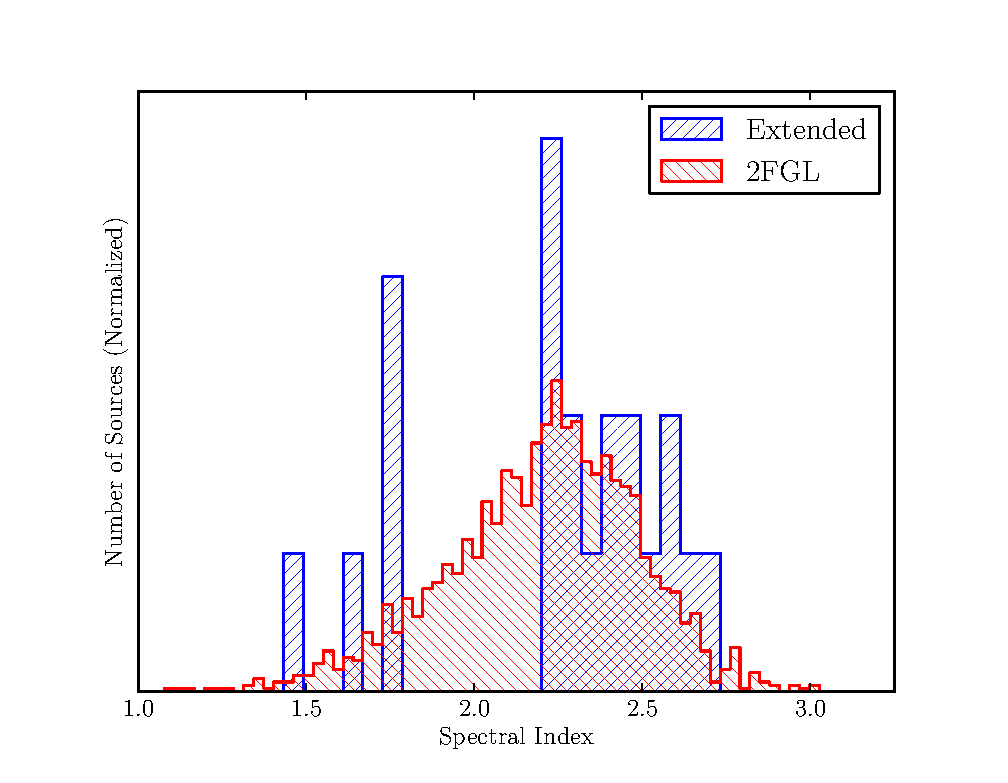
\includegraphics[scale=0.5]{../paper/summary_plots/compare_index_2FGL_color.eps}
    \column{.4\textwidth} 
    \begin{itemize}
      \item Compare Index to 2FGL 
      \item Seems like there is roughly a
        divide between softer SNRs and harder PWN
      \item Have not quantified
    \end{itemize}
  \end{columns}
\end{frame}

\begin{frame}{LAT + H.E.S.S. Sizes}
  \begin{columns}
    \column{.5\textwidth} 
    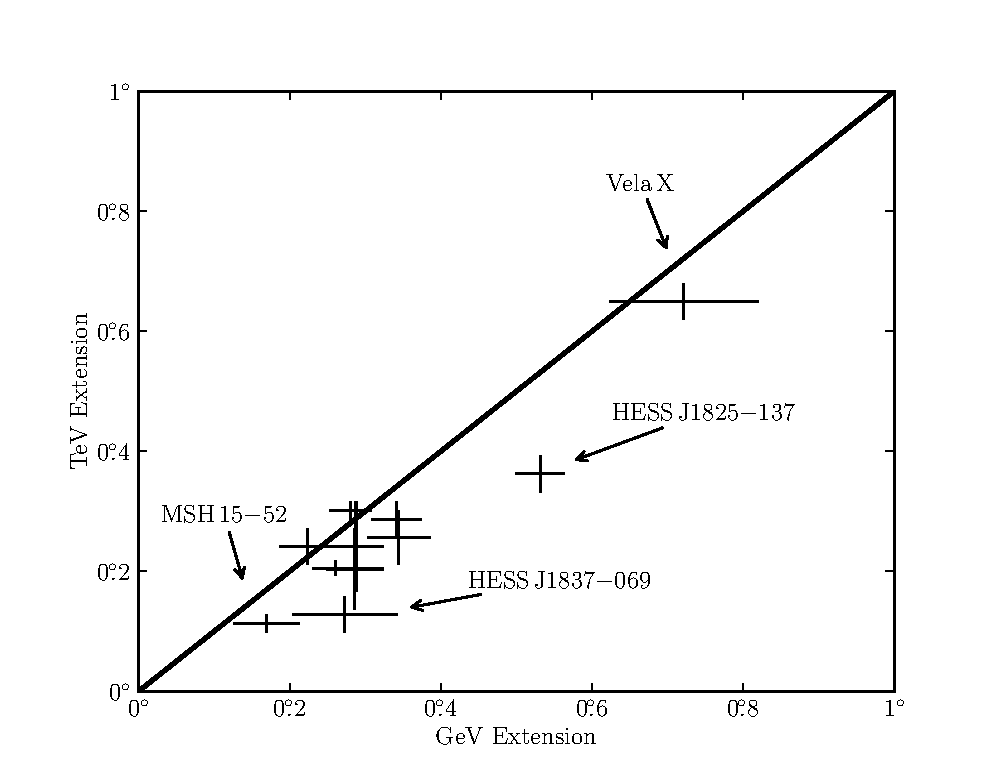
\includegraphics[scale=0.4]{../paper/summary_plots/gev_vs_tev_plot_color.eps}
    \column{.5\textwidth} 
    \begin{itemize}
      \item Compare GeV and TeV sizes
      \item Generally, good agreement
      \item HESS\,J1825$-$137 significantly
        larger at GeV than TeV
      \item Other PWN expected to be larger at
        GeV than TeV energies, but
      \item Would require improving systematics on the
        analysis (source confusion, elliptical spatial models, etc)
    \end{itemize}
  \end{columns}
\end{frame}


\begin{frame}{LAT + H.E.S.S. Distributions}
  \begin{columns}
    \column{.6\textwidth} 
    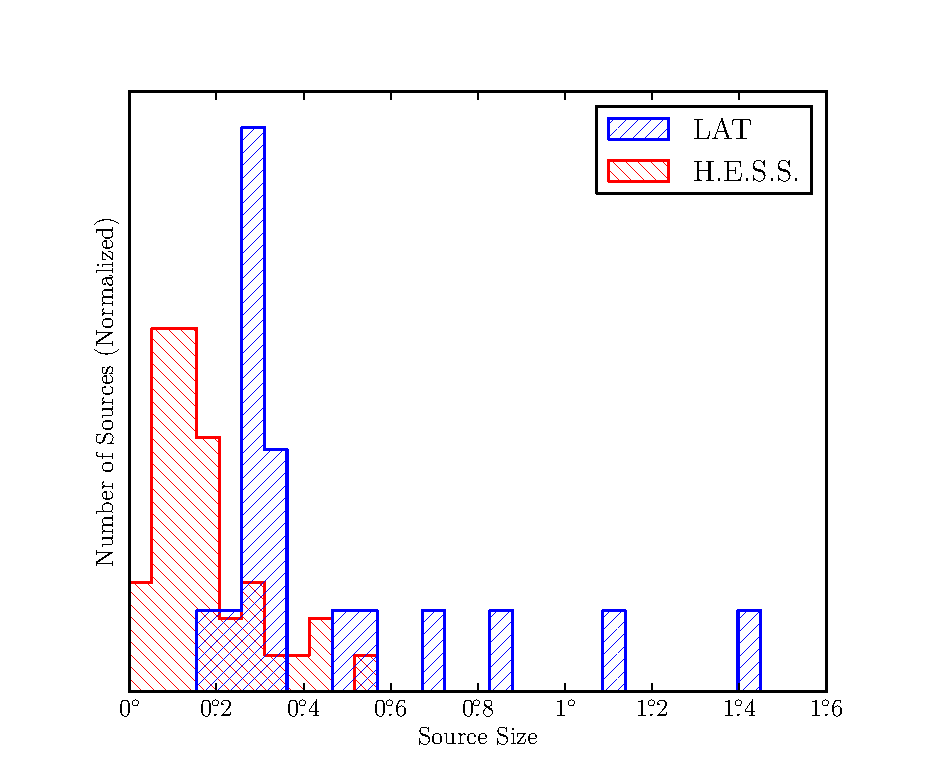
\includegraphics[scale=0.5]{../paper/summary_plots/gev_vs_tev_histogram_color.eps}
    \column{.4\textwidth} 
    \begin{itemize}
      \item Compare GeV and TeV sizes
      \item LAT detectes larger sources
      \item H.E.S.S. detects smaller sources
      \item Population of small TeV
        extended sources we can't resolve
      \item Presumably, currently outside our
        detectability
    \end{itemize}
  \end{columns}
\end{frame}

\begin{frame}{Sensitivity after 10 years}
  \begin{columns}
    \column{.6\textwidth} 
  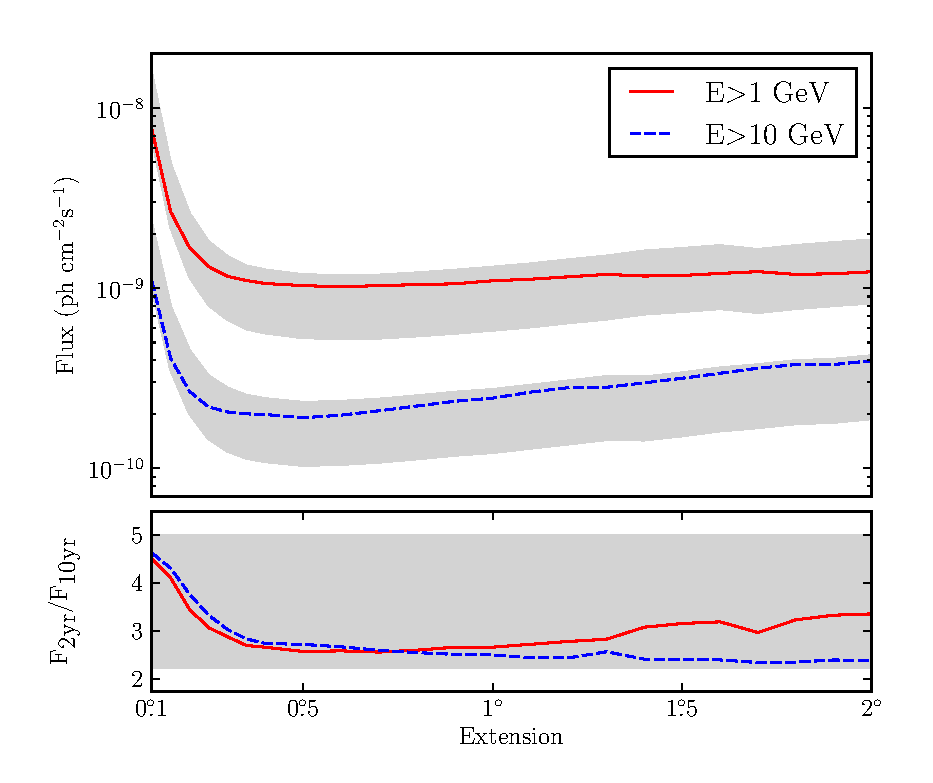
\includegraphics[scale=0.5]{../paper/mc_plots/time_sensitivity_color.eps}
    \column{.4\textwidth} 
    \begin{itemize}
      \item Calculate extension threshold with 10 year simulation
      \item Also, project from 2 year threshold by $\sqrt{time}$ and time
      \item Sensitivity $>\sqrt{time}$ for small sources
      \item Many future discoveries!
      \item Think about putting in senior review
    \end{itemize}
  \end{columns}
\end{frame}

\end{document}
